\chapter{\color{red} 任务概述}
本系统的目标是实现一个即时通讯系统,包括客户端、服务器端两个部分。

客户端主要面向工作团队用户,旨在为现代高校和企业工作团队提供一个
完整高效的即时通讯系统平台;实现通讯,管理,公告,文件的在线支持;使得
工作团队可以随时随地交流信息,协同合作;方便团队的组织和事务、活动信息
的发布;为个人资料管理和日程安排提供高效工具。

\section{目标}
实现即时通讯系统,实现需求规格说明书中所描述的一对一通讯功能、情境群聊功能、活动发布和管理功能、音视频通讯功能、通讯录功能、聊天记录功能、消息提醒功能、Board功能、个性化好友推荐功能、在线文档协作功能、日历功能、文件管理功能
和邮箱接口功能,并且保证系统健壮性和数据安全性。

\section{开发与运行环境}

\subsection{开发环境的配置}
\begin{table}[htbp]
\centering
\caption{开发环境的配置} \label{tab:development-environment}
\begin{tabular}{|c|c|c|}
    \hline
    类别 & 标准配置 & 最低配置 \\
    \hline
    计算机硬件 & \tabincell{c}{基于x86结构的CPU\\ 主频>=2.4GHz\\ 内存>=8G\\ 硬盘>=200G} & \tabincell{c}{基于x86结构的CPU\\ 主频>=1.6GHz\\ 内存>=512M\\ 硬盘>=2G} \\
    \hline
    计算机软件 & \tabincell{c}{Linux (kernel version>=4.10)\\ GNU gcc (version>=6.3.1)} & \tabincell{c}{Linux (kernel version>=3.10)\\ GNU gcc (version>=5.4)} \\
    \hline
    网络通信 & \tabincell{c}{至少要有一块可用网卡\\ 能运行IP协议栈即可} & \tabincell{c}{至少要有一块可用网卡\\ 能运行IP协议栈即可} \\
    \hline
    其他 & 采用Oracle18.3数据库 & 采用Oracle18.3数据库 \\
    \hline
\end{tabular}
% \note{这里是表的注释}
\end{table}

\subsection{测试环境的配置}

\begin{table}[htbp]
\centering
\caption{测试环境的服务器端配置} \label{tab:test-environment}
\begin{tabular}{|c|c|c|}
    \hline
    类别 & 标准配置 & 最低配置 \\
    \hline
    计算机硬件 & \tabincell{c}{基于x86结构的CPU\\ 主频>=2.4GHz\\ 内存>=128G\\ 硬盘>=200T} & \tabincell{c}{基于x86结构的CPU\\ 主频>=2.0GHz\\ 内存>=64G\\ 硬盘>=100T} \\
    \hline
    计算机软件 & \tabincell{c}{Linux (kernel version>=4.10)\\ GNU gcc (version>=6.3.1)} & \tabincell{c}{Linux (kernel version>=3.10)\\ GNU gcc (version>=5.4)} \\
    \hline
    网络通信 & \tabincell{c}{带宽>=4GB/s} & \tabincell{c}{带宽>=2GB/s} \\
    \hline
    其他 & 采用Oracle18.3数据库 & 采用Oracle18.3数据库 \\
    \hline
\end{tabular}
% \note{这里是表的注释}
\end{table}

\begin{table}[htbp]
\centering
\caption{测试环境的客户端配置} \label{tab:test-environment}
\begin{tabular}{|c|c|c|}
    \hline
    类别 & 标准配置 & 最低配置 \\
    \hline
    PC端硬件 & \tabincell{c}{Intel® Core™ i7\\ 主频>=2.0GHz\\ 内存>=8G\\ 硬盘>=200G} & \tabincell{c}{Intel® Core™ i5\\ 主频>=1.6GHz\\ 内存>=512M\\ 硬盘>=2G} \\
    \hline
    移动端硬件 & \tabincell{c}{基于armeabi-v7a架构的处理器 \\ 主频>=1.3GHz\\ 运行内存>=6G\\ 存储>=32GB} & \tabincell{c}{基于armeabi-v7a架构的处理器 \\ 主频>=0.6GHz\\ 运行内存>=512MB\\ 存储>=2GB} \\
    \hline
    网络通信 & \tabincell{c}{至少要有一块可用网卡\\ 能运行IP协议栈即可} & \tabincell{c}{至少要有一块可用网卡\\ 能运行IP协议栈即可} \\
    \hline
\end{tabular}
% \note{这里是表的注释}
\end{table}
\newpage
\subsection{运行环境的配置}

\begin{table}[htbp]
\centering
\caption{运行环境的服务器端配置} \label{tab:test-environment}
\begin{tabular}{|c|c|c|}
    \hline
    类别 & 标准配置 & 最低配置 \\
    \hline
    计算机硬件 & \tabincell{c}{基于x86结构的CPU\\ 主频>=2.4GHz\\ 内存>=128G\\ 硬盘>=200T} & \tabincell{c}{基于x86结构的CPU\\ 主频>=2.0GHz\\ 内存>=64G\\ 硬盘>=100T} \\
    \hline
    计算机软件 & \tabincell{c}{Linux (kernel version>=4.10)\\ GNU gcc (version>=6.3.1)} & \tabincell{c}{Linux (kernel version>=3.10)\\ GNU gcc (version>=5.4)} \\
    \hline
    网络通信 & \tabincell{c}{带宽>=4GB/s} & \tabincell{c}{带宽>=2GB/s}\\
    \hline
    其他 & 采用Oracle18.3数据库 & 采用Oracle18.3数据库 \\
    \hline
\end{tabular}
% \note{这里是表的注释}
\end{table}


\begin{table}[htbp]
\centering
\caption{运行环境的客户端配置} \label{tab:operation-environment}
\begin{tabular}{|c|c|c|}
    \hline
    类别 & 标准配置 & 最低配置 \\
    \hline
    PC端硬件 & \tabincell{c}{Intel® Core™ i7\\ 主频>=2.0GHz\\ 内存>=8G\\ 硬盘>=200G} & \tabincell{c}{Intel® Core™ i5\\ 主频>=1.6GHz\\ 内存>=512M\\ 硬盘>=2G} \\
    \hline
    移动端硬件 & \tabincell{c}{基于armeabi-v7a架构的处理器 \\ 主频>=1.3GHz\\ 运行内存>=6G\\ 存储>=32GB} & \tabincell{c}{基于armeabi-v7a架构的处理器 \\ 主频>=0.6GHz\\ 运行内存>=512MB\\ 存储>=2GB} \\
    \hline
    网络通信 & \tabincell{c}{至少要有一块可用网卡\\ 能运行IP协议栈即可} & \tabincell{c}{至少要有一块可用网卡\\ 能运行IP协议栈即可} \\
    \hline
\end{tabular}
% \note{这里是表的注释}
\end{table}
\newpage
\section{\color{red}需求概述}
本项目的主要功能如下:
\begin{itemize}
	\item 一对一即时通讯功能:用户可以和其他人一对一进行即时通讯。
	\item 多情境群聊功能:提供多种群聊情境,每种情境有相应的功能需求。
	\item 活动/任务发布与管理功能:在群聊中或Board上发布的任务、活动信息可以加入个人日程。
	\item 音视频通话(会议)功能:可以进行一对一或多人即时音视频通话。
	\item 通讯录功能:每个用户可以有自己的通讯录。
	\item 聊天记录功能:系统可以维护用户的聊天记录。
	\item 消息提醒功能:系统可以提示用户新的信息。
	\item Board(广场)功能:用户可以发布日志并阅读别的用户发表的日志。
	\item 个性化好友推荐功能:系统可以为用户推荐好友人选。
	\item 在线文档协作平台功能:用户可以在线共同编辑文档。
	\item 账号保护和隐私保护功能:系统可以保护用户信息。
	\item 日历管理功能:用户可以管理自己的日历。
	\item 个人本地和云端文件管理功能:用户可以通过软件管理本地或云端的文件。
	\item 邮箱接口功能:用户可以借助第三方邮箱插件管理邮箱。
	\item \color{red} 第三方账号同步功能:用户可以获得第三方账号 (github,LinkedIn,其他社交软件) 的消息更新提醒并浏览消息内容
	\item \color{red} 信息调研功能:用户可以发起调研,控制参与调研的人员,获取调研结果
	\item \color{red} 流程审批功能:用户可以发起审批申请,上传相关信息和材料,审批信息将会通知到审批人账号,可以在线审批,随时查看审批进度
\end{itemize}

{\color{red} 对应的需求图如下:}
\newpage
\begin{figure}[ht]
            \centering
            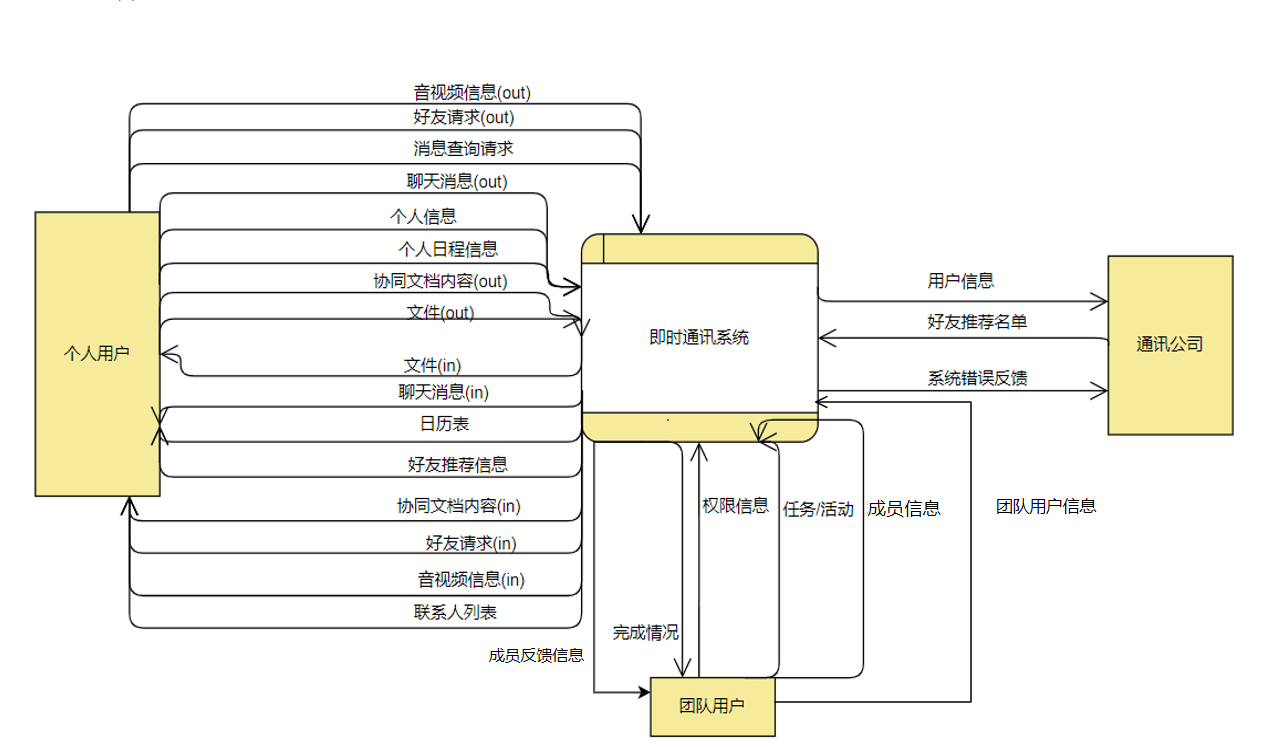
\includegraphics[scale = 0.9]{总体需求.png}\label{tab:classification}
            \caption{\color{red} 需求概念图}\label{fig:noted-figure}
        \end{figure}

\section{条件与限制}
\subsection{技术}
即时通讯系统的主要功能是提供现代工作场景下信息
交互,通知发布,团队组织、任务管理的平台解决方案。所依赖的的安卓、IOS、
Windows、Linux 操作系统,Intel 和智能移动端硬件平台,JAVA 开发语言和 Eclipse
开发环境都是成熟的开发生态圈,技术上可行。
\subsection{成本}
经济可行性上,本团队人力成本相对大型互联网企业偏低,场地使用学校实
验室不需要支付额外的费用,开发除了硬件消耗,服务器租用,软件维护的少量
费用以外,不存在其余开发费用。启动资金在个人承受范围以内,经营成本相对
低。通过广告、融资之后硬件和人力经济压力也会有所缓解, 因此经济上具有可
行性。
\subsection{法律}
即时通讯系统需要保障数据安全与用户隐私,具有法律上的责任。
本项目不侵犯任何其他工作的专利权和版权,具有法律可行性。
